 % -*- root: ../main.tex -*-
\documentclass[../main.tex]{subfiles}
\begin{document}

\chapter{Publications}\label{chap:publications}

\clearpage
\newpage

% ================================================

\glsresetall
\section{Mécanismes d'action des récepteurs aux hormones thyroïdiennes durant le développement : Lessons retenues des études sur les amphibiens}\label{sec:bba-review}

\begin{abstractfr}
Les \glspl{tr} jouent un rôle critique durant le développement des vertébrés.
Cependant, leur mécanismes d'action \textit{in vivo} reste peu exploré.
Cette revue catalogue certains des résultats obtenus dans le contexte de la métamorphose des amphibies sur les fonctions développementales des \glspl{ht} et des \glspl{tr} et leur mécanismes associés.
\par
Un modèle de double fonction de \gls{tr} pour le développement des Anoures a été proposé il y a près d'une décade.
Selon ce modèle, \gls{tr} non lié à son ligand recrute des complexes co-répresseurs – contenant des désacétylases d'histones – au niveau de gènes cibles des \glspl{ht} durant la pré-métamorphose pour réprimer l'expression de ces gènes et empêcher la métamorphose prématurée.
Par la suite, quand les \glspl{ht} sont disponibles, \gls{tr} lié au ligand recrute des complexes co-activateurs – contenant des modificateurs d'histones et des remodeleurs de la chromatine – pour cette fois activer l'expression de ces même gènes et induire les changements associés à la métamorphose.
Ces complexes peuvent altérer la structure de la chromatine par déplacement ou éviction des nucléosomes et la modification d'histones, contribuant au recrutement de la machine transcriptionnelle et à l'activation de gènes.
\par
Les mécanismes moléculaires impliqués dans ce modèle sont très probablement transposables à des modèles mammaliens.
\end{abstractfr}

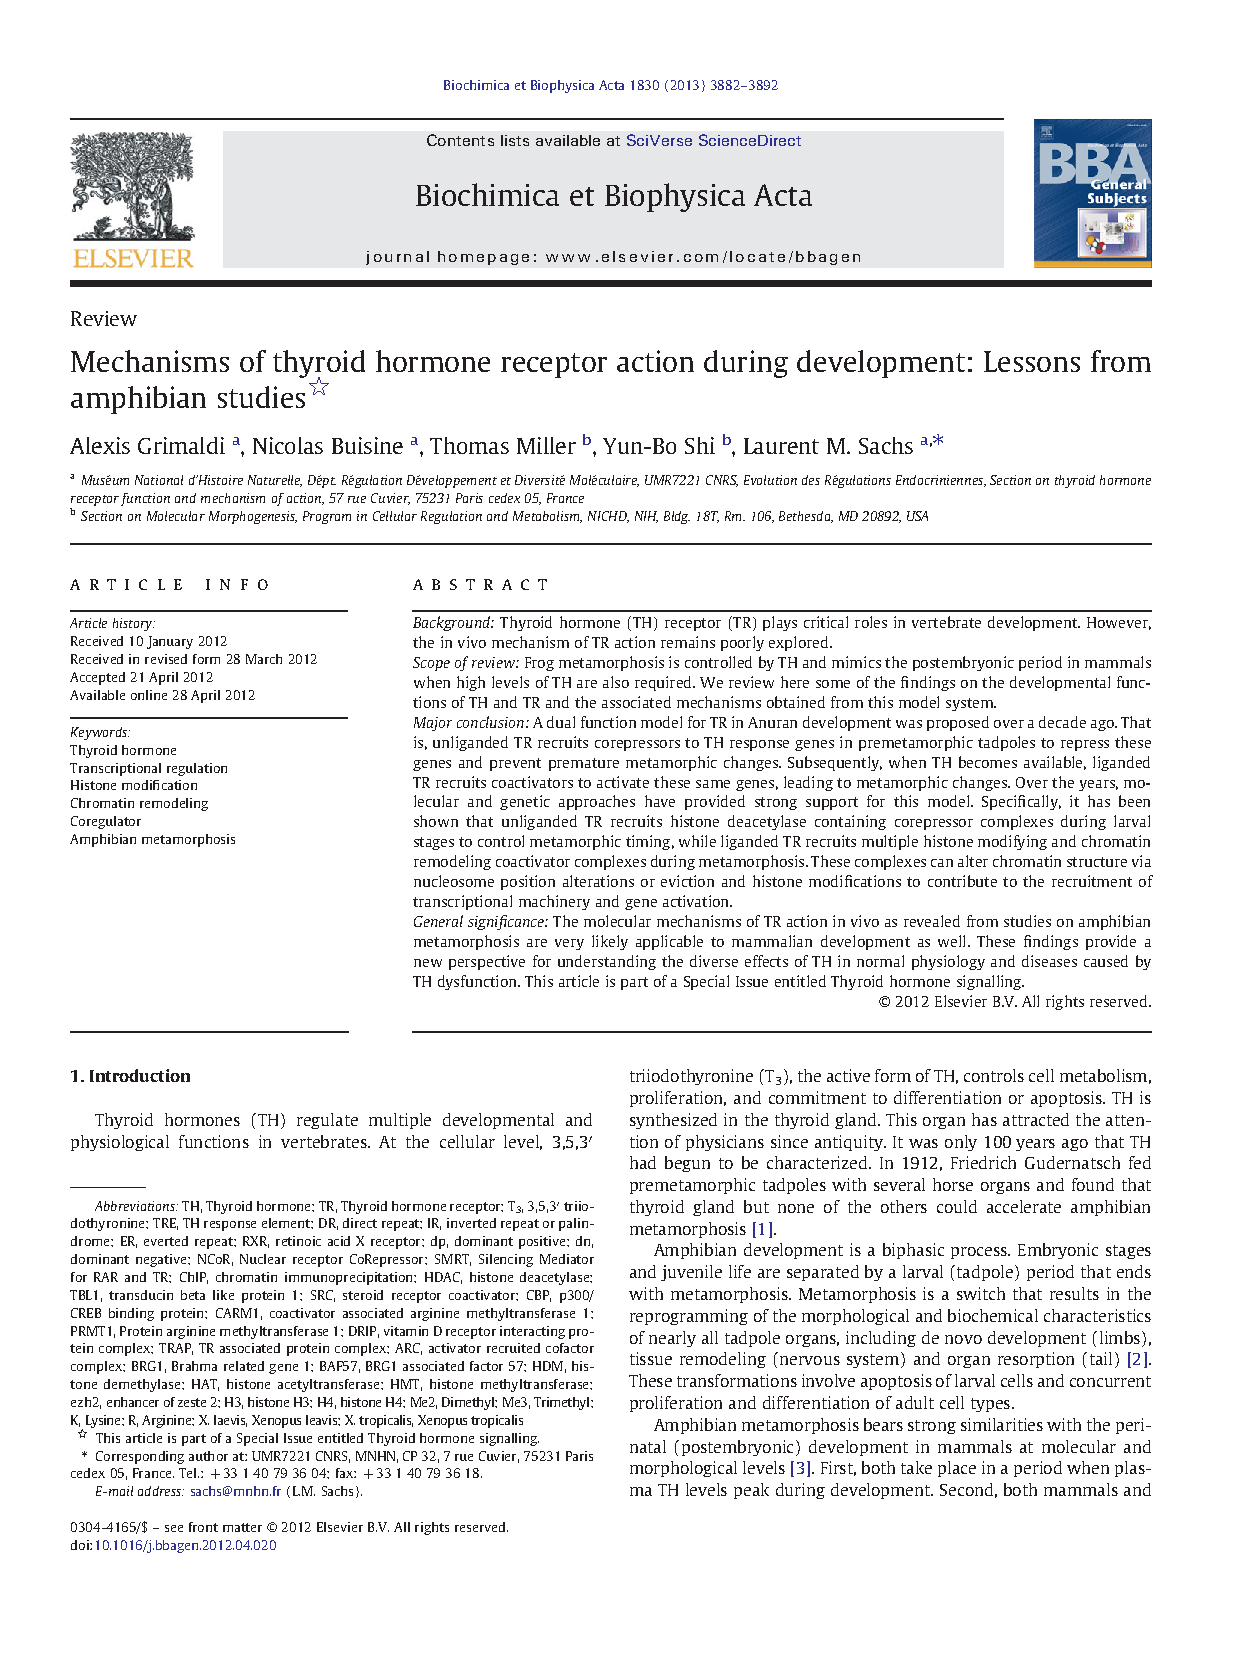
\includepdf[pages={-}]{Publications/bba-review.pdf}

% ====================================================

\clearpage
\newpage

% ====================================================

\glsresetall
\section{Les technologies de séquençage à haut débit vont métamorphoser l'analyse de la fonction des récepteurs aux hormones thyroïdiennes pendant le développement de l'amphibien}\label{sec:ctdb-review}

\begin{abstractfr}
La métamorphose des amphibiens est marquée par des changement spectaculaires induits par les \glspl{ht}, incluant de la morphogenèse, le remodelage de tissus et la résorption de tissus par mort cellulaire programmée.
\par
Les \gls{ht} agissent via leur récepteurs, les \glspl{tr}.
En absence d'hormone, ceux-ci recrutent des complexes corépresseurs au niveau des gènes cibles.
Ces complexes corépresseurs sont échangés pour des complexes coactivateurs en présence d'hormone.
Afin de pleinement comprendre la diversité des effets de la \glspl{t3} durant la métamorphose, l'analyse du transcriptome et des mécanismes d'action de \gls{tr} à l'échelle du génome est nécessaire.
\par
Les nouvelles technologies de séquençage ont profondément changé la façon dont de nouvelle questions fondamentales sont abordées, et font maintenant partie des standards utilisés en génomique et en génomique fonctionnelle.
\par
Cette revue se concentre sue les applications des nouvelles technologies de séquençage pour l'analyse et l'exploration de la métamorphose des amphibiens.
\end{abstractfr}

\iftoggle{deadtree}{
	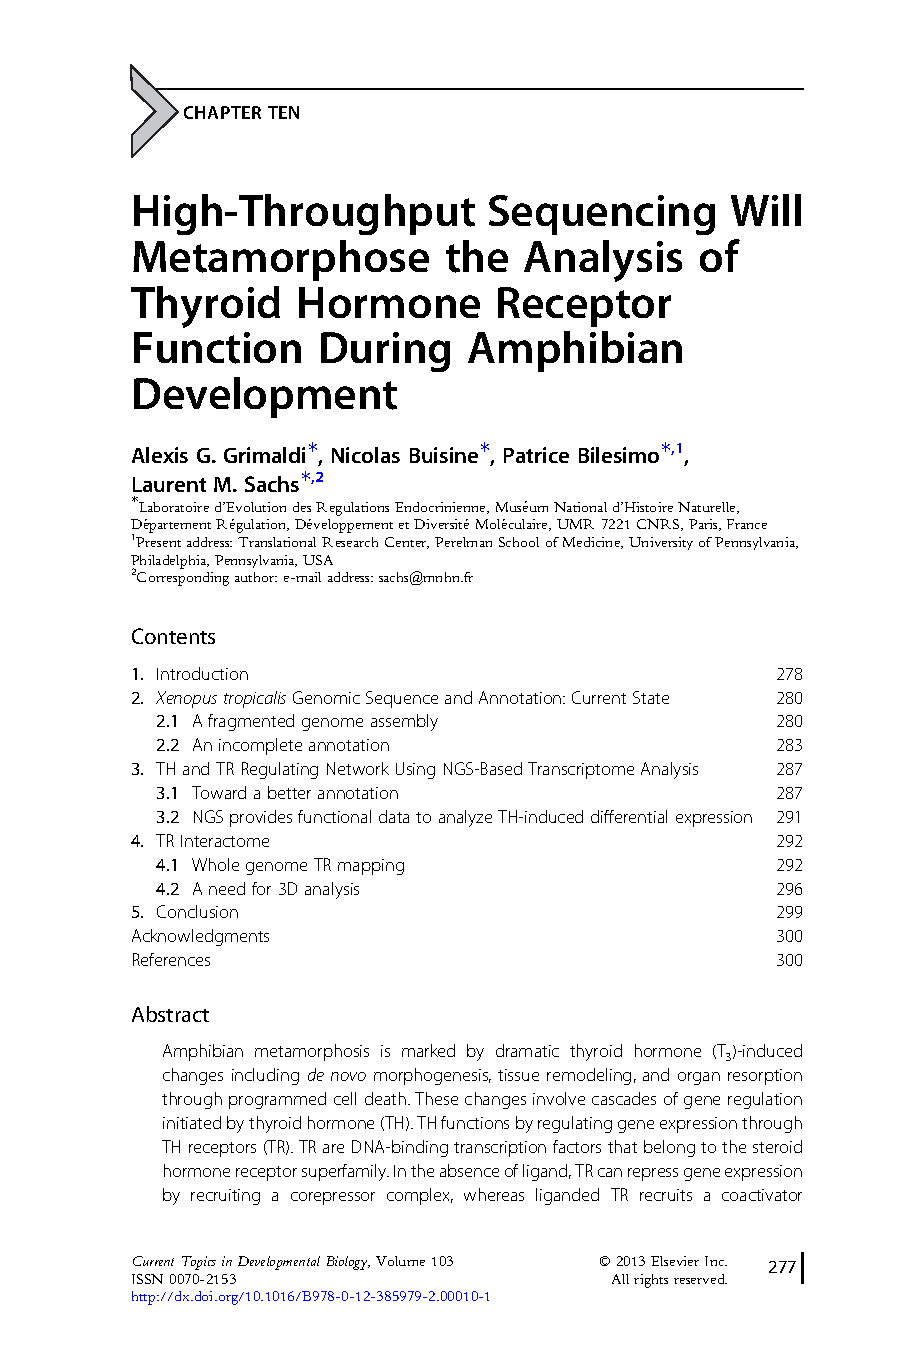
\includepdf[pages={-},nup=1x2,landscape=true]{Publications/ctdb-review.pdf}
}{
	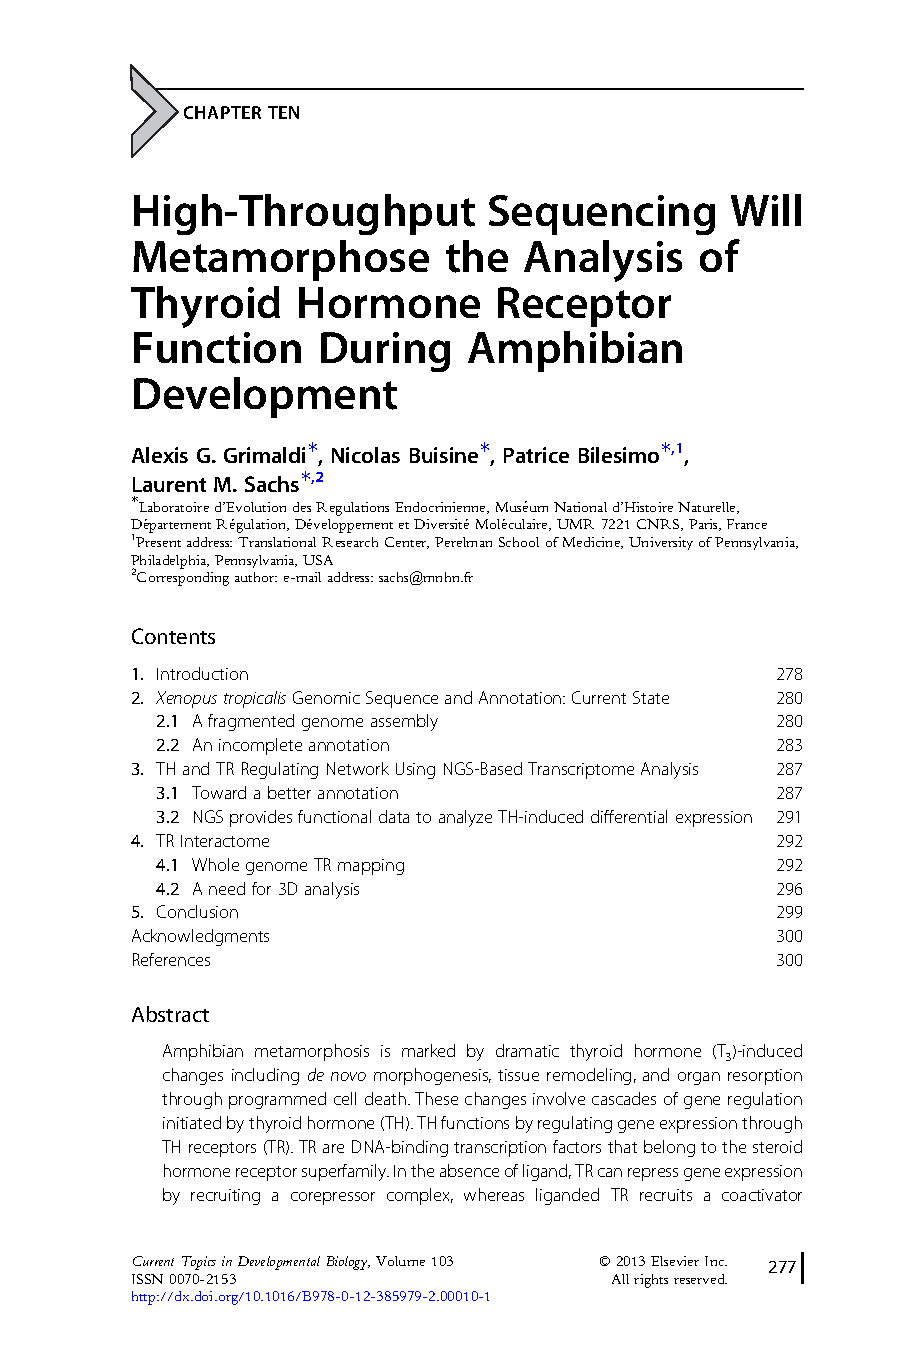
\includepdf[pages={-}]{Publications/ctdb-review.pdf}
}

\clearpage
\newpage

\glsresetall
\section{Ré-assemblage et ré-annotation du génome de \textit{X. tropicalis} pour l'analyse \textit{in vivo} de ChIA-PET}\label{sec:buisine2014}

\begin{abstractfr}
L'analyse fonctionnelle à l'échelle du génome nécessite l'annotation et l'assemblage à haute résolution de génomes.
Nous avons utilisé la technologie \gls{chiapet} pour analyser de réseaux de régulations de gènes, incluant les interactions tridimensionnelles des chromosomes qui sous-tendent la signalisation des \gls{ht} chez l'amphibien \gls{xtrop}.
Cependant, les versions actuellement disponibles de l'annotation et de l'assemblage du génome de \gls{xtrop} n'ont pas la résolution requise par le \gls{chiapet}.
Afin de surmonter ces obstacles, l'annotation et l'assemblage actuels ont été améliorés en utilisant les technologies de \gls{gpet}, \gls{rnapet}.
La grande taille (10 kb et 20 kb) des inserts utilisés pour le \gls{gpet} ont permis non seulement l'amélioration de la qualité de l'assemblage, mais également la réduction de sa fragmentation, réduisant le nombre de ``scaffolds'' de près de 60 \%.
\par
Puis, le \gls{rnaseq} a été utilisé pour capturer les transcrits pleine longueur spécifiquement au niveau de leurs extrémités $5\prime$ et $3\prime$, définissant ainsi précisément les bornes des \gls{tss} et des \gls{tts}.
Ces modifications de l'assemblage et de l'annotation ce sont révélées être des pré-requis essentiel à l'exploitation des données de \gls{chiapet}.
Cette démonstration de l'application de la technologie \gls{chiapet} pour comprendre les régulation génétiques dans un contexte physiologique chez un organisme non-conventionnel pourrait fournir des éléments de guidage méthodologiques et conceptuels pour des approches similaires chez d'autres espèces dont les données en génomique sont de basse résolution.
\end{abstractfr}

\iftoggle{deadtree}{
	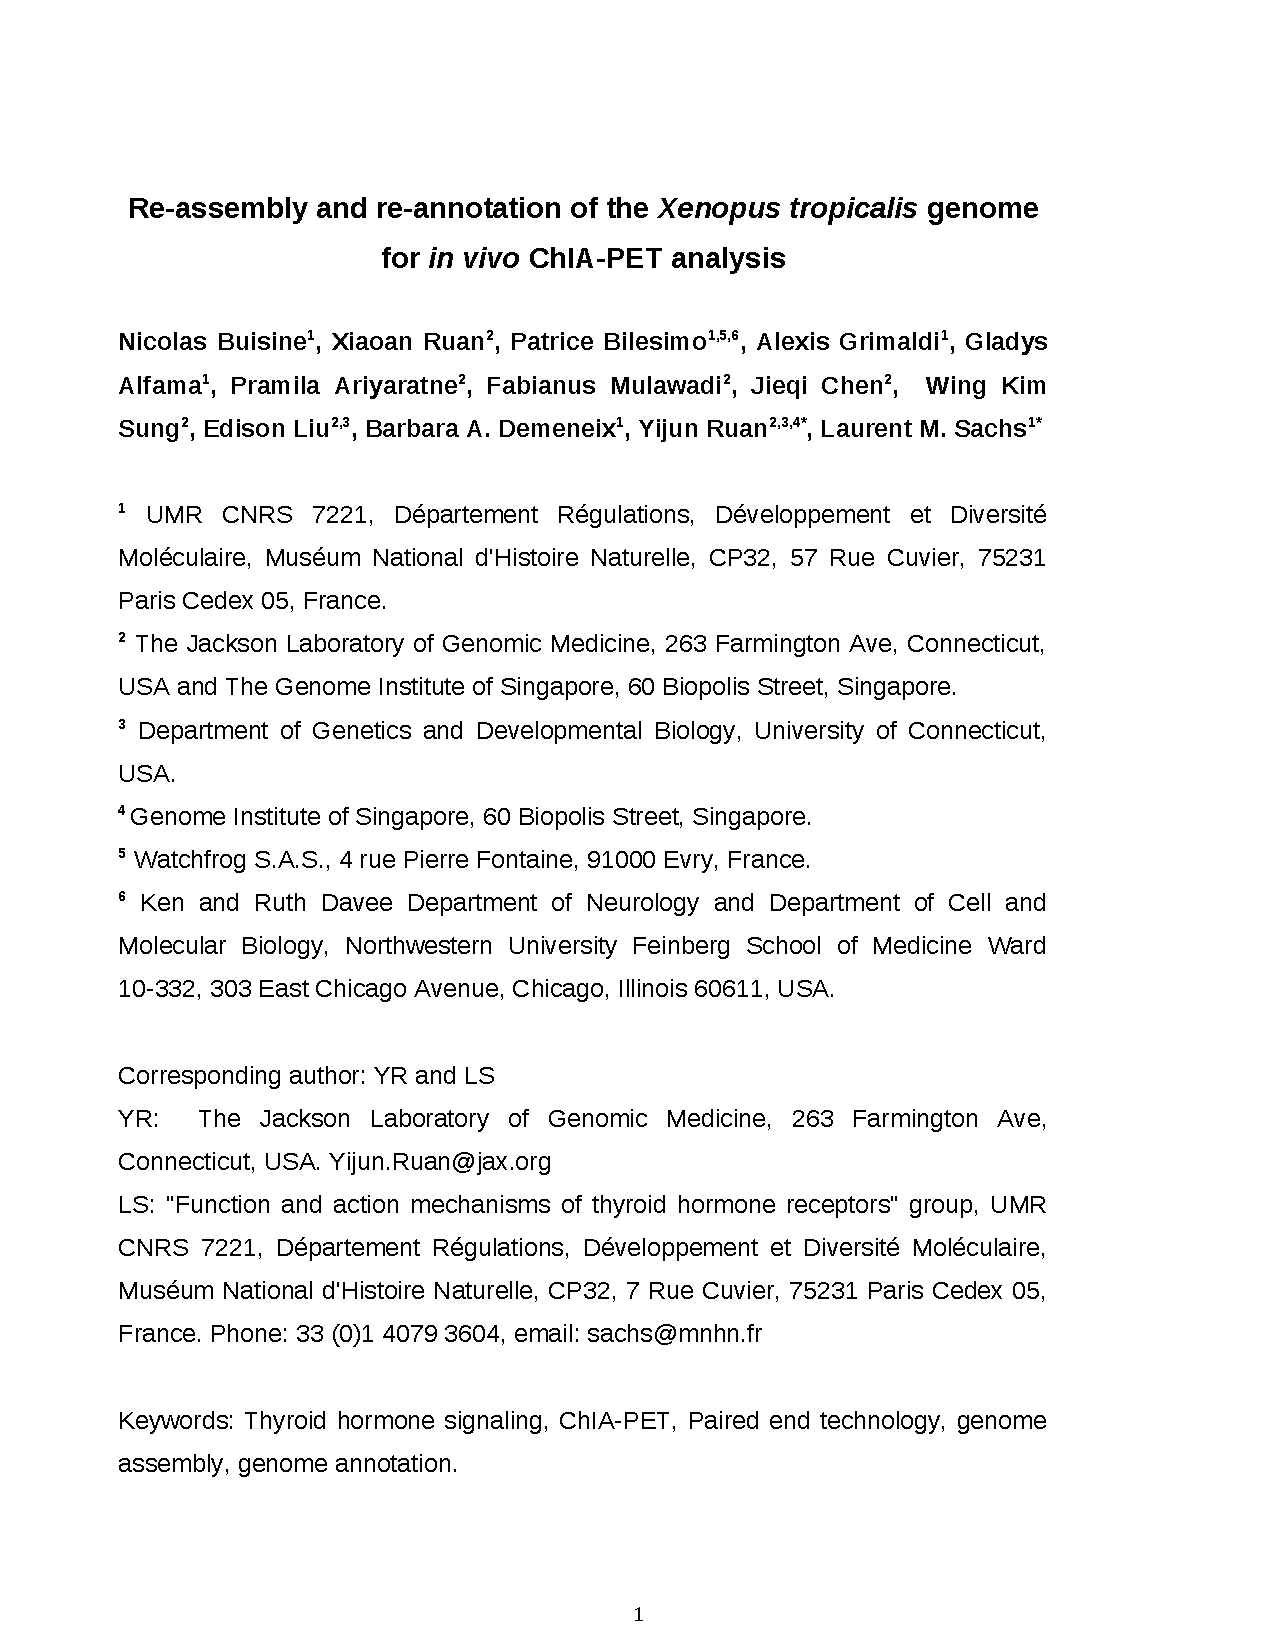
\includepdf[pages={-},nup=1x2,landscape=true]{Publications/buisine2014.pdf}
	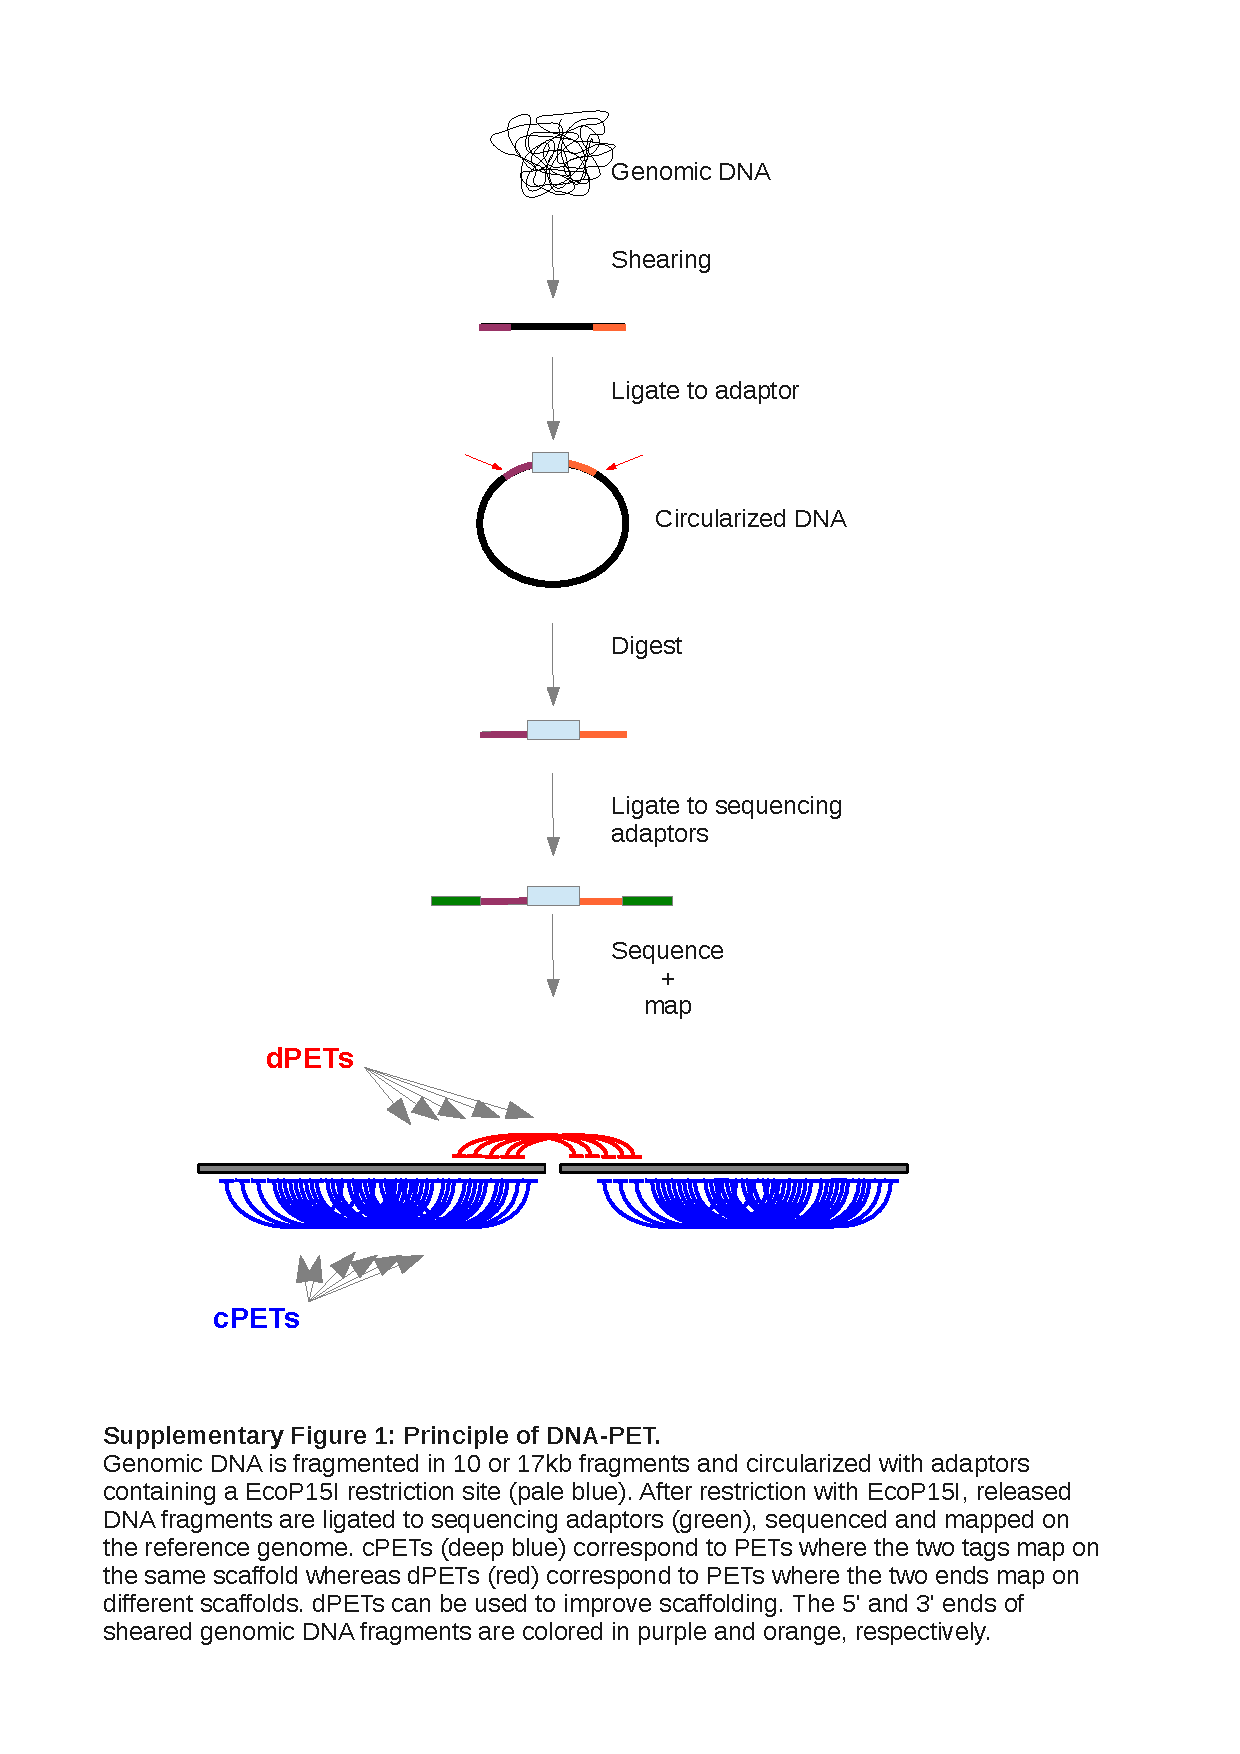
\includepdf[pages={-},nup=1x2,landscape=true]{Publications/buisine2014-sup.pdf}
}{
	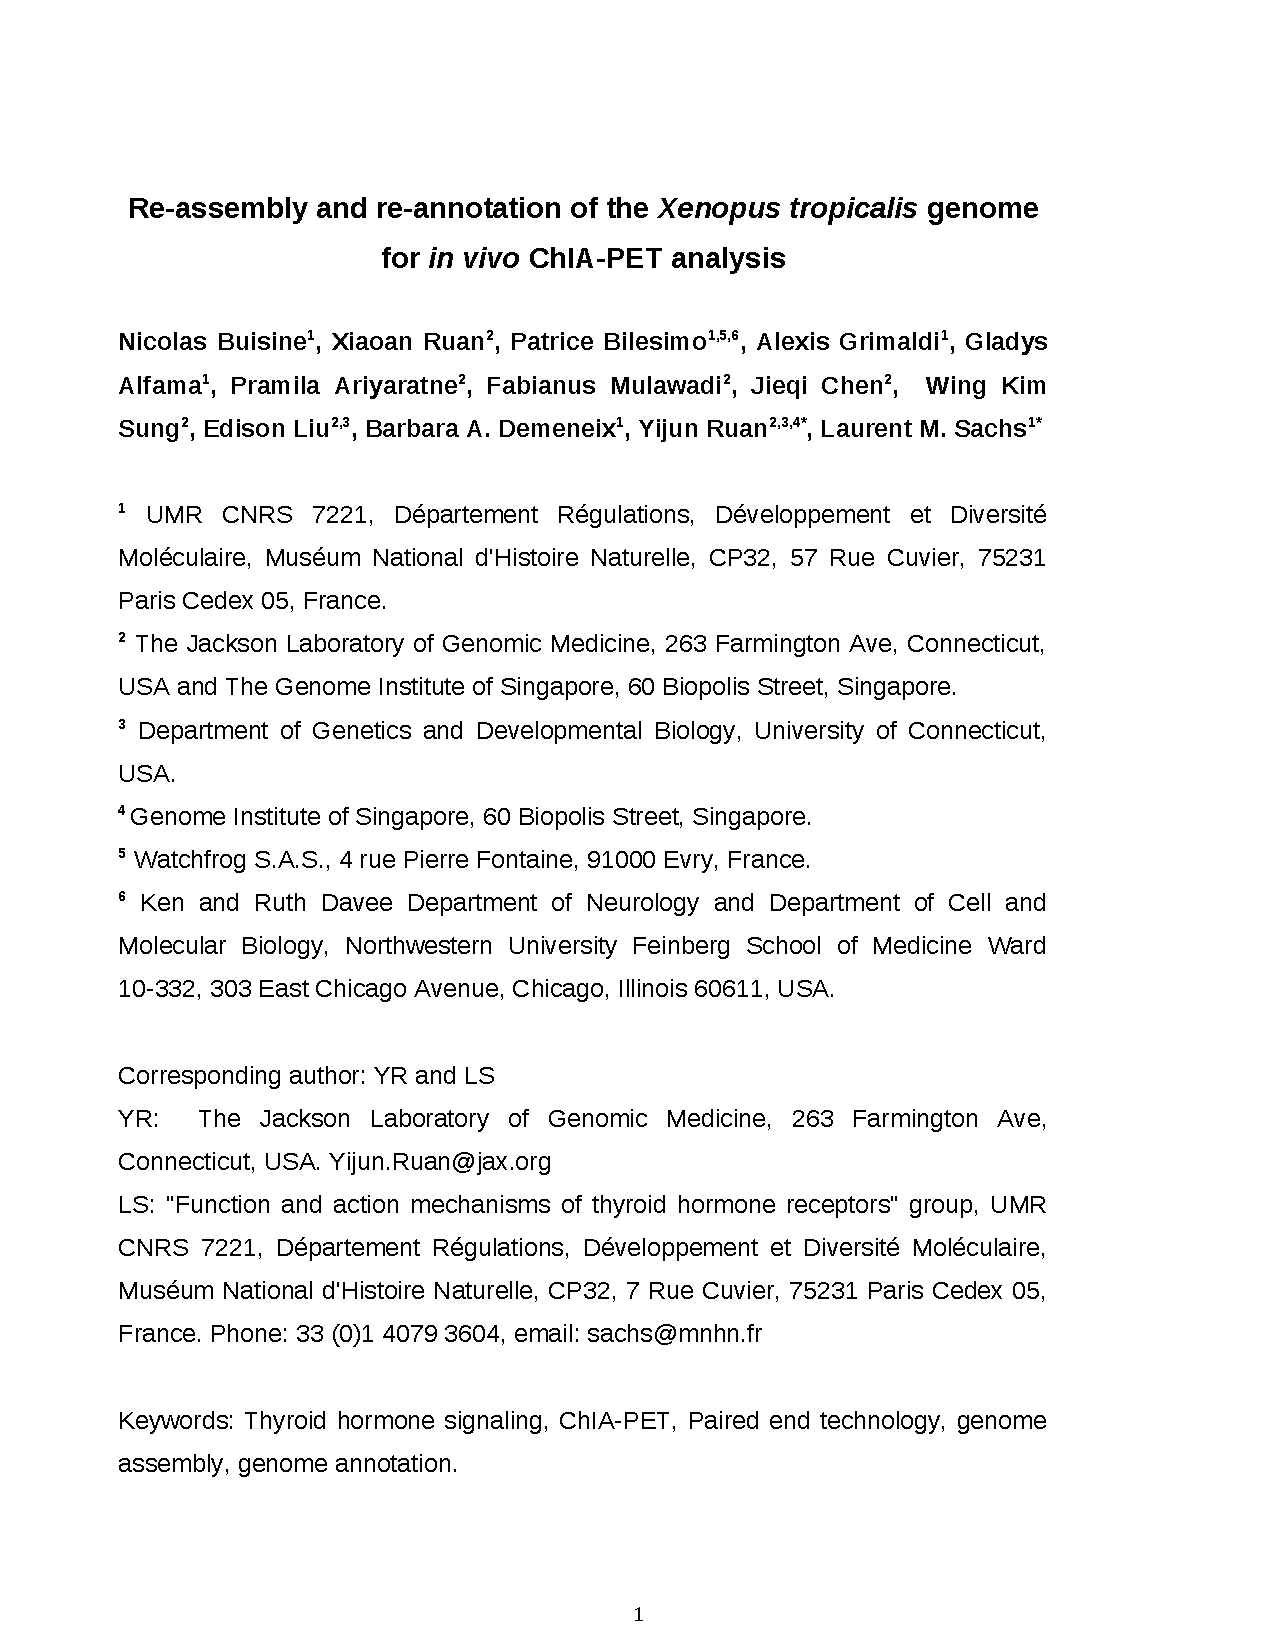
\includepdf[pages={-}]{Publications/buisine2014.pdf}
	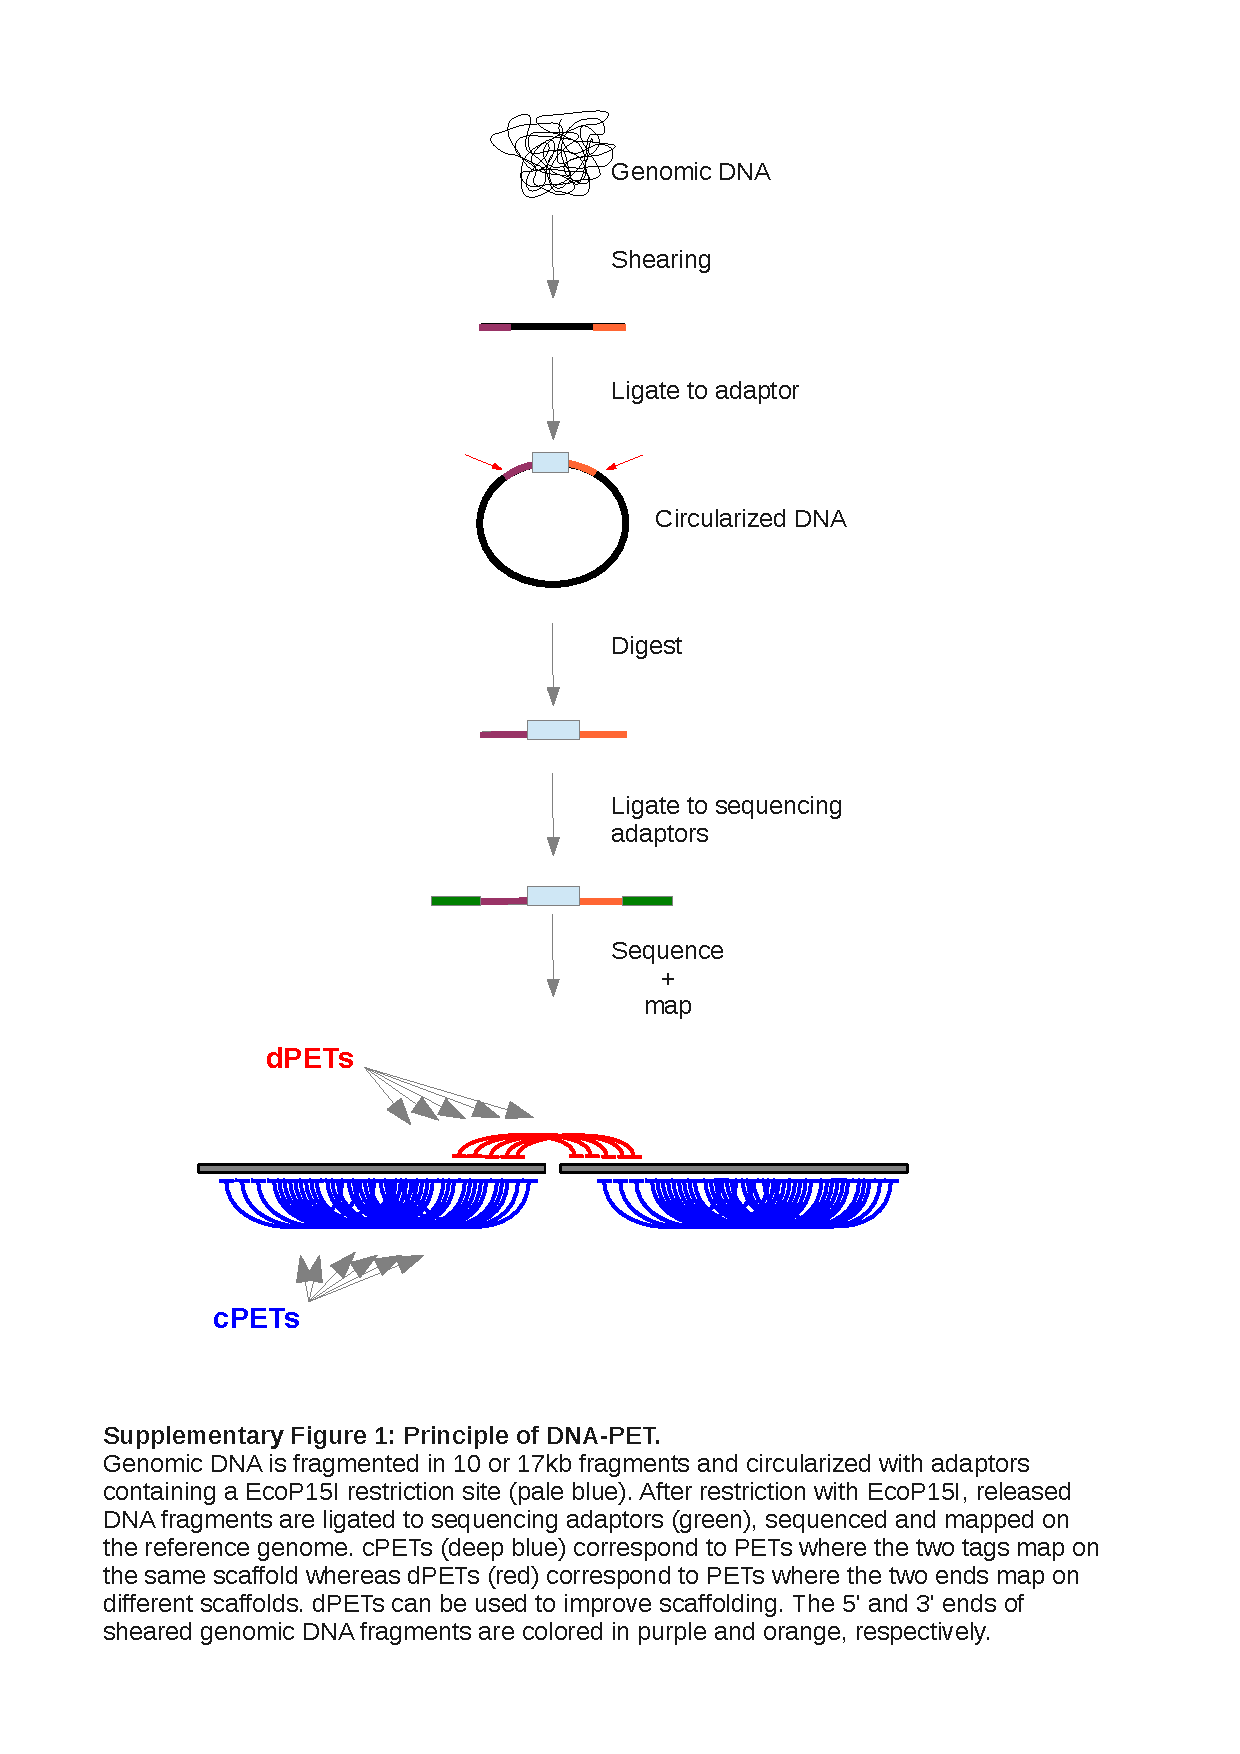
\includepdf[pages={-}]{Publications/buisine2014-sup.pdf}
}

\end{document}